%! Author = kucera-lukas
%! Date = 4/13/22

\section{Dokumentace}\label{sec:dokumentace}

Na adrese \url{https://stegoer.netlify.app/docs} se nachazí odkazy na všechny
materiály spojené s dokumentaci projektu.
Také zde můžeme nalézt odkazy ke zdrojovým kódům.

Po načtení stránky se zobrazí Accordion\cite{enwiki:accordion}.
Ten je rozdělen na 3 částí a každá odpovídá jednomu repozitáři.

\subsection{Client}\label{subsec:doc-client}
\begin{enumerate}
    \item Vývojářská dokumentace \url{https://github.com/stegoer/client/blob/master/README.md}
    \item Referenční dokumentace \url{https://stegoer.github.io/client/}
\end{enumerate}

\subsection{Server}\label{subsec:doc-server}
\begin{enumerate}
    \item Vývojářská dokumentace \url{https://github.com/stegoer/server/blob/main/README.md}
    \item Referenční dokumentace \url{https://pkg.go.dev/github.com/stegoer/server}
\end{enumerate}

\subsection{Dokumentace}\label{subsec:doc-dokumentace}
\begin{enumerate}
    \item Vývojářská dokumentace \url{https://github.com/stegoer/documentation/blob/main/README.md}
\end{enumerate}

\begin{figure}
    \centering
    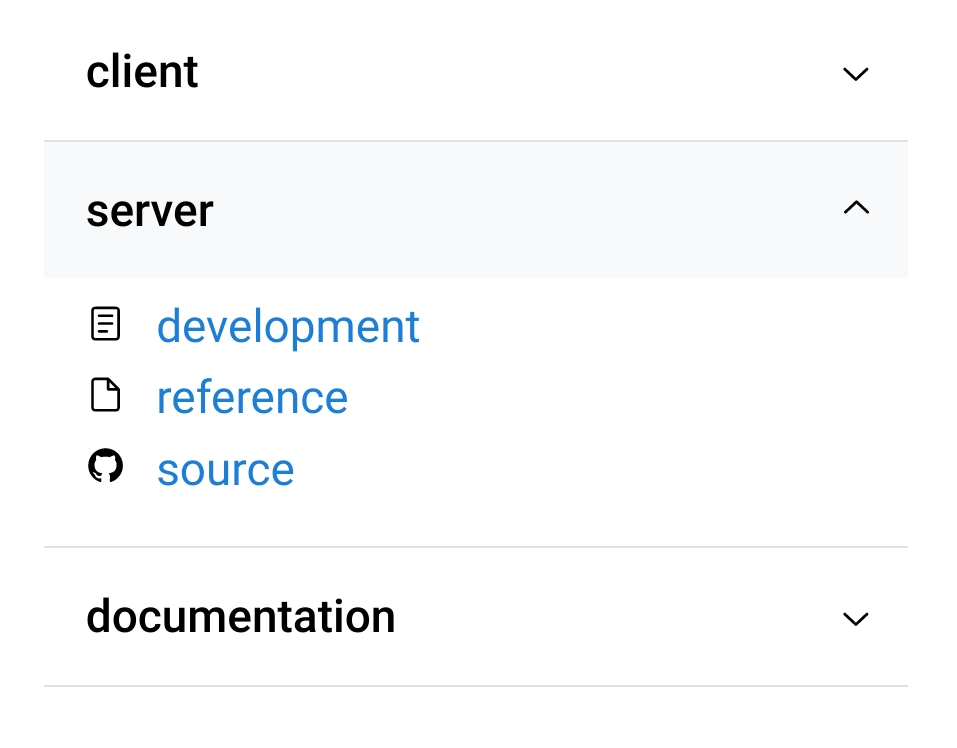
\includegraphics[scale=0.3]{assets/images/docs-accordion}
    \caption{Rozcestnik dokumentace}\label{fig:rozcestnik-dokumentace}
\end{figure}
